
When analyzing data, it can be convenient to transform the given input variables to produce new features.
For a well-chosen transform, these features may be approximated using fewer dimensions than the original input space \cite{koutroumbas2008pattern}.
This is an example of a data preprocessing technique known as \textit{dimension reduction} and can reveal low-dimensional structure.

Principal component analysis (PCA) is an orthogonal coordinate transform that is suitable for dimension reduction if some of the inputs are linearly correlated.
In this case, PCA transforms redundant variables in the input space producing uncorrelated variables in the feature space.

There are a number of ways to derive the optimal PCA transform.
One approach presented in \cite{koutroumbas2008pattern} is based on finding uncorrelated features.
It is straightforward to show that uncorrelated features have a diagonal covariance matrix.
This can be used to solve for the covariance matrix \(C\) of input variables.
By asserting the orthogonality of the PCA transform, we obtain \(V\) from the diagonalization of the covariance matrix \(C = VDV^\top\).
Given this PCA transform, we can show that \(V\) minimizes projection residuals as in \cite{shalizi2021advanced}.

\subsection{Finding uncorrelated features}
\label{sub:finding-uncorrelated-features}
The correlation between two random variables \(x\) and \(y\) is defined as
\begin{equation}
    \corr(x,y) = \frac{E[(x-\mu_x)(y-\mu_y)]}{\sigma_x \sigma_y},
\end{equation}
where \(\mu_x\), \(\mu_y\) and \(\sigma_x\), \(\sigma_y\) are the respective means and standard deviations of \(x\) and \(y\).
% If \(\mu_x = \mu_y = 0\), then we say \(x\) and \(y\) are \textit{centered}.
We say \(x\) and \(y\) are uncorrelated when \(\corr(x,y) = 0\).
This happens if and only if
\begin{equation}
    \label{eqn:covariance-formula}
    E[(x-\mu_x)(y-\mu_y)] = \cov(x,y) = 0.
\end{equation}
The covariance matrix for a multivariate random variable \(x = [x_1, x_2, \dots, x_d]\) (as a row vector) has \(\cov(x_i, x_j)\) in the \(i\)-th row and \(j\)-th column.
Then
\begin{equation}
    \label{eqn:covariance-matrix-formula}
    E[(x-\mu_x)^\top (x-\mu_x)] =
    \begin{bmatrix}
        \cov(x_1, x_1) & \cov(x_1, x_2) & \cdots & \cov(x_1, x_d) \\
        \cov(x_2, x_1) & \cov(x_2, x_2) & \cdots & \cov(x_2, x_d) \\
        \vdots         & \vdots         & \ddots & \vdots         \\
        \cov(x_d, x_1) & \cov(x_d, x_2) & \cdots & \cov(x_d, x_d) \\
    \end{bmatrix}.
\end{equation}
% If each \(x_i\) is centered, then left hand side of \cref{eqn:covariance-matrix-formula} becomes \(E(x^\top x)\).
If \(x_1, x_2, \dots, x_d\) are pairwise uncorrelated, then \(\cov(x_i, x_j) = 0\) for all \(i \neq j\).
Hence, uncorrelated variables have a diagonal covariance matrix.

Now, let \(a_1, a_2, \dots, a_n \in \RR^{1 \times d}\) represent \(n\) observations in \(d\) variables.
These observations can be considered points in \(d\)-dimensional space whose centroid is \(\mu_a = \frac{1}{n} \sum_{i=1}^{n} a_i\).
We want to determine a PCA transform which sends these points in the input space to points in the feature space.
Moreover, the basis vectors of the feature space shall be uncorrelated.
Accordingly, let \(V \in \RR^{d \times d}\) be the change of basis matrix and let
\begin{equation}
    \label{eqn:transformed-points}
    b_i = (a_i - \mu_a) V, \quad \text{for \(i = 1, 2, \dots, n\)}
\end{equation}
be observations with respect to the feature coordinates.
Then
\begin{equation}
    \mu_b
    = \frac{1}{n} \sum_{i=1}^{n} b_i
    = \frac{1}{n} \sum_{i=1}^{n} (a_i - \mu_a) V
    = 0.
\end{equation}
Using \cref{eqn:covariance-matrix-formula}, we can compute the sample covariance matrices as 
\begin{equation}
    \label{eqn:covariance-matrix-pca}
    C = \frac{1}{n-1} \sum_{i=1}^{n} (a_i - \mu_a)^\top (a_i - \mu_a),
    \qquad
    D = \frac{1}{n-1} \sum_{i=1}^{n} b_i^\top b_i.
\end{equation}
Since \(D\) is the covariance matrix of uncorrelated features, by the argument above, it is diagonal.
If we restrict \(V\) to be orthogonal, then
\begin{equation}
    \label{eqn:diagonalize-covariance}
    b_i^\top b_i = V^\top (a_i - \mu_a)^\top (a_i - \mu_a) V
    \implies
    D = V^\top C V
    \implies
    C = V D V^\top.
\end{equation}
Hence, \(V\) must be a matrix of orthonormal eigenvectors \(v_1, v_2, \dots, v_d\) corresponding to eigenvalues \(\lambda_1, \lambda_2, \dots, \lambda_d\) on the diagonal of \(D\).
When the eigenvalues and eigenvectors are ordered such that
\begin{equation}
    \lambda_1 \geq \lambda_2 \geq \cdots \geq \lambda_d,
\end{equation}
we call \(v_1, v_2, \dots, v_d\) the \textit{principal components} of the PCA transform matrix \(V\).



\subsection{Singular value decomposition}
\label{sub:singular-value-decomposition}
% TODO: SVD
The singular value decomposition (SVD) of a rectangular matrix generalizes the idea of diagonalization for square matrices.
Moreover, this provides a connection between the matrices \(A^\top A\) and \(AA^\top\).

\begin{theorem}[Singular value decomposition]
    \label{thm:svd}
    \cite{horn2013matrix}
    Let \(A \in \RR^{n \times d}\).
    Then there exist orthogonal matrices \(U \in \RR^{n \times n}\) and \(V \in \RR^{d \times d}\) and a diagonal matrix \(S \in \RR^{n \times d}\) such that \(A = USV^\top\).
    We say the columns of \(U = \begin{bmatrix}
        u_1 & u_2 & \cdots & u_n
    \end{bmatrix}\) and \(V = \begin{bmatrix}
        v_1 & v_2 & \cdots & v_d
    \end{bmatrix}\) are the left and right singular vectors of \(A\), respectively
    The diagonal entries of \(S\) are the called the singular values \(\sigma_1, \sigma_2, \dots, \sigma_r\), where \(r = \rank A \leq \min\{n,d\}\).
    Then we can write
    \begin{equation}
        \label{eqn:svd}
        A = USV^\top = \sum_{i=1}^{r} \sigma_i u_i v_i^\top.
    \end{equation}
\end{theorem}

The SVD of a matrix \(A\) can be found by diagonalizing \(A^\top A\) and \(AA^\top\).
If \(A = USV^\top\), then
\begin{align*}
    A^\top A &= (USV^\top)^\top (USV^\top) = V S U^\top U S V^\top = V S^2 V^\top\\
    AA^\top  &= (USV^\top) (USV^\top)^\top = U S V^\top V S U^\top = U S^2 U^\top.
\end{align*}

So, \(\{v_j\}_{j=1}^d\) are the eigenvectors of \(A^\top A\), \(\{u_j\}_{j=1}^n\) are the eigenvectors of \(AA^\top\), and \(\{\sigma_j^2\}_{j=1}^r\) are the eigenvalues of both \(A^\top A\) and \(AA^\top\).
Notice that the SVD of \(A\) will give us the projection matrix \(V\) in \cref{eqn:diagonalize-covariance}, provided that \(A\) is centered.
In this way, we see that PCA is really just a special case of the SVD.

\begin{theorem}[Frobenius norm]
    \label{def:frobenius}
    \cite{mohri2012foundations,horn2013matrix}
    The \textit{Frobenius norm} (or \textit{Hilbert-Schmidt norm}) of a matrix \(A = [a_{ij}] \in \RR^{n \times d}\) is given by
    \begin{equation}
        \label{eqn:frobenius}
        \|A\|_F = \sqrt{\tr(A^\top A)} = \sqrt{\sum_{i=1}^{n} \sum_{j=1}^{d} a_{ij}^2}.
    \end{equation}
\end{theorem}
\begin{proof}
    Let \(A = [a_{ij}] \in \RR^{n \times d}\).
    Then \(A^\top A = \left[\sum_{k=1}^{n} a_{k i} a_{k j}\right]_{ij}\).
    It follows that \(\|A\|_F^2 = \tr(A^\top A) = \sum_{i=1}^{n} \sum_{j=1}^{d} a_{ij}^2\).
    Clearly, \(\|A\|_F > 0\) whenever \(A\) is not the zero matrix and \(\|A\|_F = 0\) whenever \(A\) is the zero matrix.

    For the triangle inequality, consider another matrix \(B = [b_{ij}] \in \RR^{d \times m}\).
    Then
    \begin{align*}
        \|AB\|_F
        &= \sqrt{\sum_{i=1}^{n} \sum_{j=1}^{m} \sum_{k=1}^{d} (a_{ik} b_{kj})^2}\\
        &\leq \sqrt{\sum_{i=1}^{n} \sum_{j=1}^{m}
        \left(\sum_{k=1}^{d} a_{ik}^2\right) \left(\sum_{k=1}^{d} b_{kj}^2\right)}\\
        &= \sqrt{\sum_{i=1}^{n} \sum_{j=1}^{d} a_{ij}^2}
        \sqrt{\sum_{i=1}^{d} \sum_{j=1}^{m} b_{ij}^2}\\
        &= \|A\|_F \|B\|_F.
    \end{align*}
    Thus, \(\|\cdot\|_F\) is a matrix norm.
\end{proof}

Combining \cref{eqn:svd,eqn:frobenius}, we have
\begin{equation}
    \label{eqn:frobenius-singular-values}
    \|A\|_F = \sqrt{\sum_{i=1}^{r} \sigma_i^2} = \sqrt{\sum_{i=1}^{r} \lambda_i^2},
\end{equation}
where \(\{\sigma_i\}_{i=1}^r\) are the singular values of \(A\) and \(\{\lambda_i\}_{i=1}^r\) are the eigenvalues of \(A^\top A\) or \(AA^\top\).

\subsection{Minimizing projection residuals}
\label{sub:minimizing-projection-residuals}
Let \(a_1, a_2, \dots, a_n\) be points in \(\RR^d\).
Assume that these points have zero mean, that is, \(\frac{1}{n}\sum_{i=1}^{n} a_i\) is the zero vector in \(\RR^d\).
Let \(A\) be the \(n \times d\) matrix whose rows are given by \(a_1, a_2, \dots, a_n\).
Then the covariance matrix from \cref{eqn:covariance-matrix-pca} is given by \(C = \frac{1}{n-1} A^\top A\).
% \begin{align}
%     \notag
%     \|a_i - b_i\|^2
%     &= \left\langle a_i - b_i, a_i - b_i\right\rangle
%     \notag \\
%     &= \left\langle a_i, a_i \right\rangle
%     - 2\left\langle a_i, b_i \right\rangle
%     + \left\langle b_i, b_i \right\rangle
%     \notag \\
%     &= \left\| a_i \right\|^2
%     - 2\left\langle a_i, b_i \right\rangle
%     + \left\| b_i \right\|^2
%     \notag \\
%     &= \left\| a_i \right\|^2
%     - 2\left\langle a_i, \sum_{j=1}^{p} \langle a_i, v_j \rangle v_j \right\rangle
%     + \left\| \sum_{j=1}^{p} \langle a_i, v_j \rangle v_j \right\|^2
%     \notag \\
%     &= \left\| a_i \right\|^2
%     - 2\sum_{j=1}^{p} \langle a_i, v_j \rangle \left\langle a_i,  v_j \right\rangle
%     + \sum_{j=1}^{p} \langle a_i, v_j \rangle^2 \left\|  v_j \right\|^2 
%     \notag \\
%     &= \left\| a_i \right\|^2
%     - 2\sum_{j=1}^{p} \langle a_i, v_j \rangle^2
%     + \sum_{j=1}^{p} \langle a_i, v_j \rangle^2
%     \notag \\
%     \label{eqn:projection-residuals}
%     &= \left\| a_i \right\|^2
%     - \sum_{j=1}^{p} \langle a_i, v_j \rangle^2
% \end{align}

% TODO: Minimize projection residuals

% derive the first principal component by minimizing the projection residual
% derive the next principal component orthogonal to the first one that minimizes the projection residual

\subsection{PCA algorithm}
Let \(A\) be a data matrix whose \(n\) rows correspond to observations and \(d\) columns correspond to variables.
The following algorithm demonstrates a simple method for computing the PCA of \(A\):
\begin{enumerate}
    \item Compute the centered matrix \(A_0 = A - \colmean(A)\).
    \item Compute the covariance matrix \(C = \frac{1}{n-1} A_0^\top A_0\).
    \item Diagonalize the covariance matrix such that \(C = V D V^\top\).
    \item Order the eigenvalues and eigenvectors so that \(\lambda_1 \geq \lambda_2 \geq \cdots \geq \lambda_d\).
    We call the ordered eigenvalues the \textit{principal components}.
    \item Choose the dimension of the subspace \(p \leq d\).
    \item Construct the \(d \times p\) projection matrix \(V_p\) using the first \(p\) principal components \(v_1, v_2, \dots, v_p\).
\end{enumerate}

\begin{example}
    \label{eg:pca}
    % TODO: Clean up PCA example
\def\Amat{\begin{bmatrix}
    5 &  3 &  6 &  7 &  6 \\
    4 &  5 &  7 &  1 &  3 \\
    5 &  7 &  6 &  1 &  0 \\
    6 & 10 & 12 & 12 & 11 \\
    9 & 10 & 12 & 13 &  9 \\
\end{bmatrix}}
Consider the following matrix \[A = \Amat.\]
The column means are \(\mu = [5.8,7,8.6,6.8,5.8]\).
Then the mean-centered data becomes
\def\-{\phantom{-}}
\[X = A - \mu = \frac{1}{5}\begin{bmatrix}
        -4 &   -20 &   -13 &   \-1 &   \-1 \\
        -9 &   -10 &    -8 &   -29 &   -14 \\
        -4 &   \-0 &   -13 &   -29 &   -29 \\
        \-1 &  \-15 &  \-17 &  \-26 &  \-26 \\
    \-16 &  \-15 &  \-17 &  \-31 &  \-16 \\
\end{bmatrix}.\]

The covariance matrix is
\[C = X^TX = \frac{1}{5}\begin{bmatrix}
        74 &  85 &  93 & 179 & 104 \\
        85 & 190 & 170 & 225 & 150 \\
        93 & 170 & 196 & 313 & 238 \\
    179 & 225 & 313 & 664 & 484 \\
    104 & 150 & 238 & 484 & 394 \\
\end{bmatrix}.\]

Diagonalizing \(C\) gives
\begin{align*}
    V &= \begin{bmatrix}
        0.1888 & -0.2020 & -0.6366 &  0.5495 & -0.4651\\
        0.2755 & -0.7886 &  0.1472 & -0.4502 & -0.2791\\
        0.3606 & -0.3464 &  0.3128 &  0.5836 &  0.5582\\
        0.6979 &  0.2522 & -0.4422 & -0.3707 &  0.3411\\
        0.5209 &  0.3922 &  0.5288 &  0.1316 & -0.5271\\
    \end{bmatrix},\\
    D &= \begin{bmatrix}
        264.8458 &       0 &      0 &      0 & 0 \\
                0 & 27.9766 &      0 &      0 & 0 \\
                0 &       0 & 9.3198 &      0 & 0 \\
                0 &       0 &      0 & 1.4579 & 0 \\
                0 &       0 &      0 &      0 & 0 \\
    \end{bmatrix}.
\end{align*}

If we keep all \(5\) principal component vectors, then \(V_5 = V\) and the projection of \(X\) along \(V\) is
\[P = XV = \begin{bmatrix}
    -1.9469 &  4.3453 & -0.8756 & -0.2039 & 0 \\
    -6.9742 & -0.0660 &  1.4352 &  0.7590 & 0 \\
    -8.1577 & -2.6752 & -0.8063 & -0.5704 & 0 \\
        8.4282 & -0.2330 &  1.8282 & -0.4996 & 0 \\
        8.6507 & -1.3711 & -1.5815 &  0.5149 & 0 \\
\end{bmatrix}.\]
Here, the last column of \(P\) is the zero vector because the last eigenvalue of \(C\) is zero\footnote{Since we subtracted the column means from a square matrix \(A\), the dimension of the row space was reduced to 4.}.
To perfectly reconstruct \(A\), we need \(k = 4\) principal components and the row vector \(\mu\)
\[A = PV^T + \mu = PV_4^T + \mu.\]

If we use \(k = 3\) principal components, then the projection of \(X\) onto \(V_3\) is
\[P = XV_3 = \begin{bmatrix}
    -1.9469 &  4.3453 & -0.8756 \\
    -6.9742 & -0.0660 &  1.4352 \\
    -8.1577 & -2.6752 & -0.8063 \\
        8.4282 & -0.2330 &  1.8282 \\
        8.6507 & -1.3711 & -1.5815 \\
\end{bmatrix}\]
and \(A\) is approximately reconstructed by
\[A \approx P V_3^T + \mu = \begin{bmatrix}
    % 5.1121 &  2.9082 &  6.1190 &  6.9244 &  6.0268 \\
    % 3.5829 &  5.3417 &  6.5570 &  1.2814 &  2.9001 \\
    % 5.3134 &  6.7432 &  6.3329 &  0.7886 &  0.0751 \\
    % 6.2745 &  9.7751 & 12.2916 & 11.8148 & 11.0658 \\
    % 8.7170 & 10.2318 & 11.6995 & 13.1909 &  8.9322 \\
    5.1 &  2.9 &  6.1 &  6.9 &  6.0 \\
    3.6 &  5.3 &  6.6 &  1.3 &  2.9 \\
    5.3 &  6.7 &  6.3 &  0.8 &  0.1 \\
    6.3 &  9.8 & 12.3 & 11.8 & 11.1 \\
    8.7 & 10.2 & 11.7 & 13.2 &  8.9 \\
\end{bmatrix}.\]
We can compute the reconstruction error using
\begin{equation*}%\label{eqn:reconstruction_error}
    E_k = \|A - (PV_k^T + \mu)\|_F,
\end{equation*}
where \(\|\cdot\|_F\) is the Frobenius norm.
By the SVD, we have \(X = USV^T\), where \(S = \sqrt{D}\).
So, the projection of \(X\) onto \(V_k\) is \[P = XV_k = US_k,\] where \(S_k\) is the diagonal matrix of the first \(k\) singular values.
Then the reconstruction error becomes
\begin{align*}
    \|A - (PV_k^T + \mu)\|_F
    &= \|(A - \mu) - PV_k^T\|_F \\
    &= \|X - PV_k^T\|_F \\
    &= \|USV^T - US_kV^T\|_F \\
    &= \|U(S - S_k)V^T\|_F \\
    &= \|S-S_k\|_F \\
    &= \sigma_k + \sigma_{k+1} + \dots + \sigma_{p}.
\end{align*}
Hence,
\[E_3 = \sigma_3 + \sigma_4 = \sqrt{1.4579} + 0 = 1.2074.\]
\end{example}

\subsection{Applications of PCA}

One of the most common applications of PCA is \textit{dimension reduction}.
When variables are correlated, the observations lie in some linear subspace of the original space.
In this situation, PCA can be used to project down to the lower dimension and have the smallest possible projection error.
This is particularly useful when the dimension of the input space is extremely large.
A number challenges arise when analyzing high-dimensional data and are collectively referred to as the \textit{curse of dimensionality} \cite{koutroumbas2008pattern}.
By working in the PCA feature space, these problems may be avoided.

\begin{example}
    \label{eg:pca-code}
    \begin{figure*}
    \centering
    \makebox[\textwidth][c]{%
    \begin{minipage}{6.5in}
        \centering
        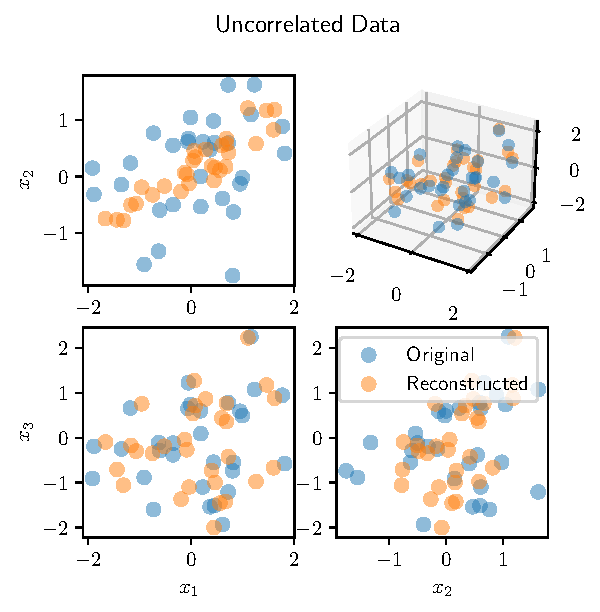
\includegraphics[width=.49\textwidth]{figs/fig-pca-code-uncorr.pdf}
        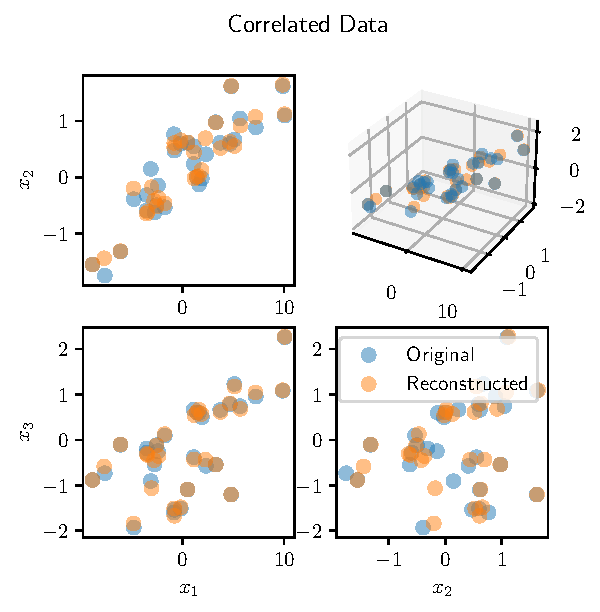
\includegraphics[width=.49\textwidth]{figs/fig-pca-code-corr.pdf}
    \end{minipage}}
    \caption{PCA projection of three-dimensional data onto two-dimensional subspace.}
    \label{fig:pca-code}
\end{figure*}
In the following experiment, we consider two sets of three-dimensional data.
Each set of vectors \(x_1, x_2, x_3 \in \RR^n\) are sampled from a standard normal distribution with sample size \(n = 30\).
Suppose in the first set there is no apparent relationship among variables while, in second set, we have \(x_1 = 4x_2 + 2x_3\).
For simplicity, we say the first set is \textit{uncorrelated} while the second set is \textit{correlated}.
See \Cref{fig:pca-code}.
In the uncorrelated data, the reconstruction error is \(~ 3.92\), which does not seem to indicate the presence of a pattern.
The reconstruction error for the correlated data is \(~ 0.973\).
This error can be explained by the variation of \(x_2\) with \(x_3\).
Meanwhile, the correlated pair plots indicate a pattern among \(x_2\) vs \(x_1\) and \(x_3\) vs \(x_1\).
\end{example}

% \subsection{Linear regression and PCA}
% \def\vb#1{\mathbf{#1}}
\cite{shawe2004kernel}
Let \(\vb{x}_1, \dots, \vb{x}_m \in \RR^n\) be observation vectors and \(\vb{y} \in \RR^n\) be a target vector.
A linear regression model finds a vector of weights \(\vb{w} = (w_1, w_2, \dots, w_n)\) to determine the linear function
\begin{equation}
    f(\vb{x}) = \vb{w} \cdot \vb{x} = \sum_{i=1}^{n} w_i x_i,
\end{equation}
where \(\vb{x} = (x_1, x_2, \dots, x_n)\) is an input vector.
The residual error of each observation is \(\vb{y} - f(\vb{x}_i)\), for \(i = 1,2, \dots, m\).
Then the residual sum of squares is given to be
\begin{equation}
    \label{eqn:residual-sum-of-squares}
    RSS
    = \sum_{i=1}^{m} (\vb{y} - f(\vb{x}_i))^2
    = \sum_{i=1}^{m} (\vb{y} - \vb{w} \cdot \vb{x}_i)^2
    = (\vb{y} - X^\top \vb{w})^\top (\vb{y} - X^\top \vb{w}),
\end{equation}
where \(X = [\vb{x}_1, \dots, \vb{x}_m]\).
By minimizing \(RSS\), the magnitude of the residuals will be as small as possible, producing the optimal linear model \(f(\vb{x})\).
Therefore, this method is known as least squares regression.
Differentiate \eqref{eqn:residual-sum-of-squares} with respect to \(\vb{w}\) and set equal to zero so that
\begin{equation}
    2 X^\top \vb{y} - 2 X^\top X \vb{w} = 0.
\end{equation}
This leads to the normal equation \(X^\top X \vb{w} = X^\top \vb{y}\).
Thus,
\begin{equation}
    \vb{w} = (X^\top X)^{-1} X^\top \vb{y}
\end{equation}
gives the optimal linear model which minimizes residual error.

% \begin{example}
%     
In two dimensions, let \(\vb{x} = (x_1, \dots, x_m)\) and \(\vb{y} = (y_1, \dots, y_m)\).
Then the least squares regression model is given by
\begin{equation}
\label{eqn:ols-model}
f(x) = \frac{\cov(\vb{x},\vb{y})}{\Var(\vb{x})}(x - \overline{\vb{x}}) + \overline{\vb{y}},
\end{equation}
Since \(\vb{x}\) is treated as an input variable and \(\vb{y}\) is treated as an output, this is a type of supervised learning.
In contrast, PCA is an unsupervised learning technique.
PCA organizes the variables in the input space to reveal any patterns in the underlying data.
% \footnote{I think this model would be considered total least squares (TLS) regression since it uses all variables (input and output). Principal component regression (PCR) creates the regression equation using only the input variables.}
If we have input variables \(\vb{x}_1\) and \(\vb{x}_2\), we can use PCA to find a linear pattern among the inputs without trying to predict an output.
First, we find the direction of the largest variance \(\lambda_{\max}\) using the covariance matrix
\[\begin{bmatrix}
\cov(\vb{x}_1, \vb{x}_1) & \cov(\vb{x}_1, \vb{x}_2) \\
\cov(\vb{x}_2, \vb{x}_1) & \cov(\vb{x}_2, \vb{x}_2)
\end{bmatrix} = \begin{bmatrix}
\Var(\vb{x}_1) & \cov(\vb{x}_1, \vb{x}_2) \\
\cov(\vb{x}_1, \vb{x}_2) & \Var(\vb{x}_2)
\end{bmatrix}.\]
In particular,
\[\lambda_{\max} = \frac{1}{2}\left(\Var(\vb{x}) + \Var(\vb{y}) + \sqrt{(\Var(\vb{x}) - \Var(\vb{y}))^2 + 4\cov(\vb{x},\vb{y})^2}\right).\]
Then the PCA regression model becomes
\begin{equation}
\label{eqn:pca-model}
g(x) = \frac{\lambda_{\max} - \Var({\vb{x}_1})}{\cov(\vb{x}_1,\vb{x}_2)}(x - \overline{\vb{x}}_1) + \overline{\vb{x}}_2.
\end{equation}
In this case, the projection residuals are orthogonal to the PCA regression line.
See \Cref{fig:ols-pca}.

\begin{figure}
\centering
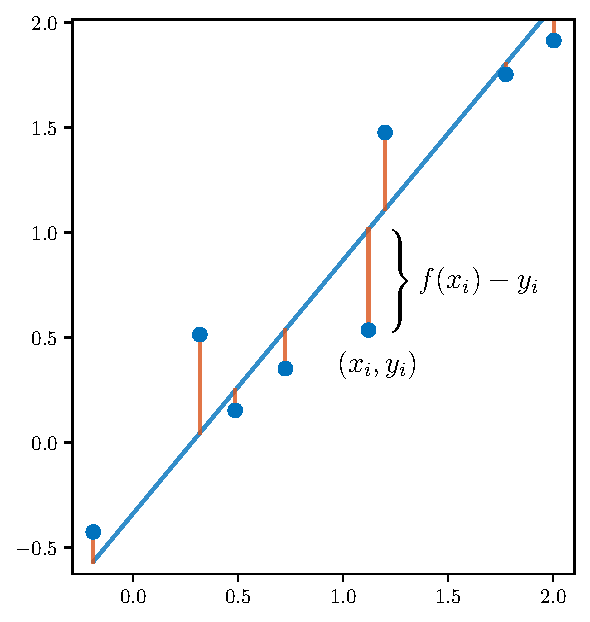
\includegraphics[width=.49\linewidth]{figs/fig-least-squares.pdf}
\hfill
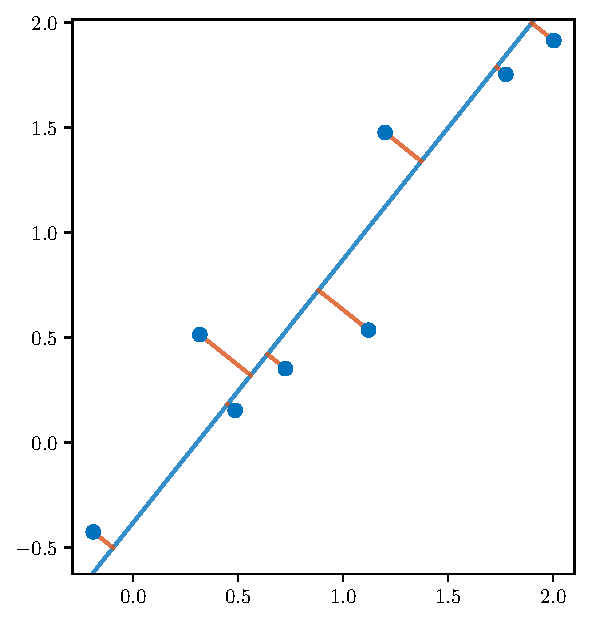
\includegraphics[width=.49\linewidth]{figs/fig-pca-fit.pdf}
\caption{Least squares regression model \(f(x)\) (left) minimizes the sum of squared errors while total least squares, i.e., the PCA model \(g(x)\) (right) minimizes the orthogonal projections.}
\label{fig:ols-pca}
\end{figure}
% \end{example}